\documentclass[journal]{IEEEtran}

\usepackage{graphicx}
\usepackage{amsmath}
\usepackage{booktabs}
\usepackage{url}

\title{Simulation-Based Implementation of Lean Manufacturing Techniques for Productivity Improvement: An Expanded Data-Driven Case Study From a Beverage Bottling Line}

\author{
    Your Name
    \thanks{Your Name is with the Department of Production and Industrial Engineering, Your University, Your City, India. Replace this line with your actual name, university, and affiliation before submission.}
}

\begin{document}

\maketitle

\begin{abstract}
Lean manufacturing is widely recognized as an effective strategy for reducing waste and improving productivity, yet many small and medium-sized manufacturing firms still face difficulty in deciding which lean techniques should be implemented first. This problem becomes more significant when companies have limited resources and cannot afford repeated trial-and-error implementation on the shop floor. This paper develops an expanded, data-driven simulation framework to evaluate lean interventions using a real industrial production dataset from a beverage bottling line monitored through an Industrial Internet of Things (IIoT) system. The dataset contains 59 production summary records across 56 calendar production days between July 22, 2022 and February 6, 2023, 265 hourly operating observations, and 1,388 downtime events. First, the production system is studied through throughput, availability, downtime, product mix, and temporal variability. Next, downtime events are classified into micro-, minor-, and major-stoppage categories to identify the dominant source of waste. Finally, an event-level bootstrap simulation is used to evaluate three lean scenarios: 5S with visual management, total productive maintenance (TPM), and an integrated lean bundle. The baseline system produced 212,358 liters with an observed availability of 42.66\%. Downtime analysis shows that micro-stoppages account for 61.31\% of all events but only 13.59\% of downtime minutes, while major stoppages represent only 6.77\% of events but consume 66.26\% of total downtime minutes. Simulation results show that 5S and visual management improve output by 2.33\%, TPM improves output by 20.61\%, and an integrated lean bundle improves output by 32.19\%, while raising mean simulated availability from 42.37\% to 55.33\%. The main implication is that maintenance-led reduction of major stoppages should be prioritized before broad workplace-stabilization efforts when downtime severity is highly concentrated. The study contributes a reproducible open-data framework for simulation-based lean analysis and provides a stronger final-year-project template for SME-oriented manufacturing research.
\end{abstract}

\begin{IEEEkeywords}
Lean manufacturing, productivity improvement, bottling line, downtime analysis, discrete-event simulation, SMEs, total productive maintenance, 5S, IIoT, digital manufacturing.
\end{IEEEkeywords}

\section{Introduction}
Lean manufacturing has remained one of the most influential improvement philosophies in industrial engineering because it aims to eliminate non-value-added activity while improving flow, quality, and responsiveness. In production systems with unstable operation, the practical challenge is not whether lean is useful, but which lean technique should be prioritized first. This challenge becomes more serious for SMEs and small-scale operations, where technical staff, budgets, and improvement time are limited. A wrong implementation sequence can consume management attention without delivering meaningful productivity gains.

Several prior studies have shown that lean practices can improve operational performance in manufacturing systems [1]. However, the effect of lean tools is not uniform. Some interventions produce only incremental gains in one context but much larger gains in another. Simulation therefore becomes valuable because it provides a low-risk decision environment where lean alternatives can be tested before physical implementation [3], [5].

Recent work has also shown that lean manufacturing and smart manufacturing are increasingly complementary rather than contradictory. Digital data can improve the diagnosis of waste, the measurement of flow losses, and the design of targeted interventions [6], [10]. At the same time, the literature on simulation in SMEs still emphasizes the need for more practical, accessible, and reproducible approaches [3].

This paper addresses that need by using a real open industrial dataset from a beverage bottling line [8]. The dataset is particularly useful because it contains production summaries, hourly operating information, and a large event-level downtime log collected through an IIoT architecture associated with industrial production forecasting research [7]. Using these data, the present study develops a reproducible simulation-based evaluation of lean interventions.

The paper contributes in four ways:
\begin{enumerate}
    \item it translates a real industrial dataset into a lean-analysis workflow;
    \item it quantifies the relative importance of downtime frequency versus downtime severity;
    \item it compares alternative lean strategies through simulation rather than intuition alone; and
    \item it offers an expanded IEEE-style manuscript that can be adapted into a student project report or conference paper.
\end{enumerate}

\section{Literature Review and Research Gap}
Belekoukias \emph{et al.} [1] showed that lean methods and tools can improve operational performance, but they also emphasized that the magnitude of improvement depends on implementation context. Oleghe and Salonitis [2] argued that quantitative lean evaluation still needs stronger modeling treatment, especially when human and production interactions create complex dynamic behavior. Yu and Chen [3] reviewed factory simulation in SMEs and concluded that simulation is useful but still under-adopted, partly because SMEs need more targeted and easier-to-transfer applications.

Later studies confirmed that simulation can help select lean techniques rather than merely document them after implementation. Possik \emph{et al.} [4] proposed a co-simulation framework for evaluating lean techniques in manufacturing systems and showed that different lean tools have different leverage depending on system structure. Frecassetti \emph{et al.} [5] used simulation in an Italian SME and demonstrated that simulation supports better prioritization of lean interventions before implementation.

At the same time, digital manufacturing research has started to strengthen lean analysis. Bokhorst \emph{et al.} [6] showed that smart manufacturing often builds directly on lean principles. Reslan \emph{et al.} [10] further demonstrated that digital twins can automate value stream mapping and strengthen lean diagnostics. In food and beverage SMEs, Matindana and Shoshiwa [9] found that lean implementation is relevant and beneficial, but empirical studies in this area still remain limited.

Despite these advances, three gaps remain:
\begin{enumerate}
    \item Many lean-simulation studies use proprietary industrial datasets, limiting reproducibility.
    \item Many lean studies report improvement conceptually, but do not connect event-level downtime data to scenario-based simulation.
    \item SME-relevant manufacturing sectors such as food and beverage still have fewer open, data-driven lean case studies than high-tech or automotive sectors.
\end{enumerate}

The present study addresses these gaps by integrating real downtime-event data, lean scenario design, and simulation-based productivity analysis in a fully reusable workflow.

\begin{table}[!t]
\caption{Literature Synthesis and Research Gap}
\label{tab:litgap}
\centering
\begin{tabular}{p{2.6cm}p{3.2cm}p{2.2cm}}
\toprule
Study & Main Contribution & Remaining Gap \\
\midrule
[3] Yu and Chen & Review of simulation use in SMEs & Need more practical and transferable SME cases \\
[4] Possik \emph{et al.} & Co-simulation for lean impact evaluation & Limited open-data reproducibility \\
[5] Frecassetti \emph{et al.} & Lean-practice selection in an SME & Case data not openly reusable \\
[6] Bokhorst \emph{et al.} & Lean-smart manufacturing connection & Does not test downtime-driven lean scenarios \\
[10] Reslan \emph{et al.} & Digital twin value stream mapping & Limited direct productivity simulation evidence \\
This study & Open-data, downtime-driven lean simulation & Reproducible SME-relevant framework \\
\bottomrule
\end{tabular}
\end{table}

\section{Problem Definition and Mathematical Formulation}
The line under study experiences significant downtime variability. The main research problem is to determine which lean strategy produces the best productivity improvement under actual operating variability. The analysis uses the following performance relationships.

\subsection{Availability}
\begin{equation}
A = \frac{T_{op}}{T_{mon}}
\end{equation}
where $A$ is operational availability, $T_{op}$ is effective operating time, and $T_{mon}$ is monitored time.

\subsection{Downtime}
\begin{equation}
T_{dt} = T_{mon} - T_{op}
\end{equation}
where $T_{dt}$ is downtime or pause time.

\subsection{Production Rate}
\begin{equation}
R = \frac{Q}{T_{op}}
\end{equation}
where $Q$ is total output in liters and $R$ is liters produced per operating hour.

\subsection{Scenario-Based Output}
\begin{equation}
Q' = R(T_{mon} - T'_{dt})
\end{equation}
where $Q'$ is simulated output under a lean scenario and $T'_{dt}$ is scenario-adjusted downtime.

\subsection{Downtime Transformation}
\begin{equation}
T'_{dt} = T_{res} + \sum_{i=1}^{n}\alpha_i t_i
\end{equation}
where $T_{res}$ is residual downtime not captured as event records, $t_i$ is downtime event $i$, and $\alpha_i$ is the reduction factor assigned to that event category.

\subsection{Output Improvement}
\begin{equation}
\%\Delta Q = \frac{Q' - Q}{Q}\times 100
\end{equation}

\section{Dataset and Methodology}
\subsection{Dataset Description}
The dataset used in this study is the \emph{Industrial Production Time-Series Dataset from a Beverage Bottling Line} released on Zenodo on January 4, 2026 [8]. The data span July 22, 2022 to February 6, 2023 and include multiple sheets describing hourly production, daily production summaries, hourly operation breakdown, and downtime-event logs. The associated IIoT production-forecasting article confirms the industrial nature of the data source and the digital acquisition context [7].

The main dataset characteristics are summarized in Table~\ref{tab:dataset}.

\begin{table}[!t]
\caption{Dataset Characteristics}
\label{tab:dataset}
\centering
\begin{tabular}{lr}
\toprule
Attribute & Value \\
\midrule
Monitoring period & Jul.\ 22, 2022 to Feb.\ 6, 2023 \\
Production summary records & 59 \\
Calendar production days & 56 \\
Hourly operating observations & 265 \\
Downtime events & 1,388 \\
Observed product sizes & 3 L and 5 L \\
Total liters produced & 212,358 \\
Total monitored time & 238.65 h \\
\bottomrule
\end{tabular}
\end{table}

\subsection{Analytical Procedure}
The study follows six steps:
\begin{enumerate}
    \item clean and read the production and downtime sheets;
    \item aggregate daily and hourly operating metrics;
    \item classify downtime events into micro, minor, and major categories;
    \item estimate empirical production rates from the real observations;
    \item build an event-level bootstrap simulation with 5,000 replications; and
    \item compare scenario performance using output, availability, and pause-time reduction.
\end{enumerate}

\subsection{Downtime Classification}
Downtime events are categorized as follows:
\begin{itemize}
    \item \textbf{Micro-stoppages:} $t \leq 2$ min
    \item \textbf{Minor stoppages:} $2 < t \leq 10$ min
    \item \textbf{Major stoppages:} $t > 10$ min
\end{itemize}

This classification is useful because it separates frequent short flow interruptions from low-frequency high-impact breakdowns.

\subsection{Simulation Design}
The simulation uses bootstrap resampling at the day level. Each replication samples the observed day profiles with replacement and keeps the original production-rate structure. Event durations are first normalized to match recorded daily pause time, ensuring that the baseline simulation is consistent with the actual system. Lean interventions are then imposed as counterfactual changes in downtime occurrence or downtime duration.

Three scenarios are modeled:
\begin{enumerate}
    \item \textbf{5S + Visual Management:} 15\% of micro-stoppages are removed.
    \item \textbf{TPM:} major stoppage durations are reduced by 25\%.
    \item \textbf{Integrated Lean Bundle:} 20\% of micro-stoppages are removed, minor stoppages are reduced by 15\%, and major stoppages are reduced by 30\%.
\end{enumerate}

These percentages are scenario assumptions informed by lean literature and operational logic. They are not post-implementation measurements.

\section{Results and Visual Analysis}
\subsection{Baseline System Performance}
The line produced 212,358 liters from 60,888 units during 238.65 monitored hours. Effective operating time was only 101.81 hours, while pause time reached 137.56 hours, resulting in an observed overall availability of 42.66\%. This confirms that downtime, rather than nominal line capacity, is the main constraint in the system.

At the product level, the average production rate was 1,963.71 L/h for the 3 L product and 2,918.68 L/h for the 5 L product. At the date-aggregated level, pause time had a strong negative correlation with efficiency ($r=-0.707$), which supports the use of downtime reduction as the primary improvement lever.

\begin{table}[!t]
\caption{Baseline Performance Indicators}
\label{tab:baseline}
\centering
\begin{tabular}{lr}
\toprule
Metric & Value \\
\midrule
Production days & 56 \\
Production summary records & 59 \\
Hourly observations & 265 \\
Downtime events & 1,388 \\
Total production & 212,358 L \\
Total units produced & 60,888 \\
Monitored time & 238.65 h \\
Operating time & 101.81 h \\
Pause time & 137.56 h \\
Overall availability & 42.66\% \\
\bottomrule
\end{tabular}
\end{table}

\begin{figure}[!t]
\centering
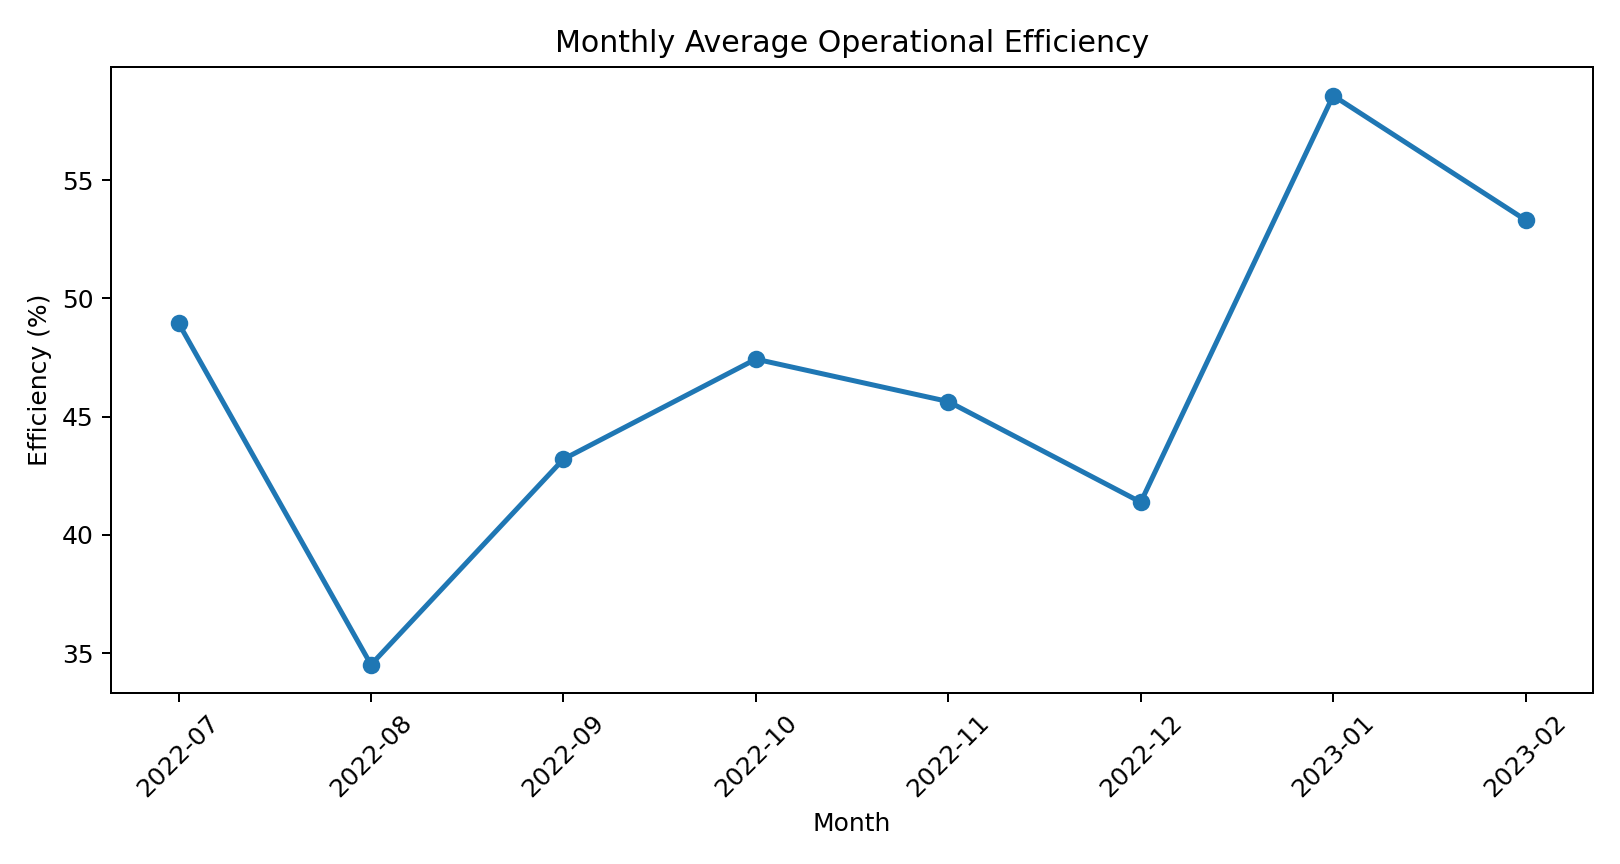
\includegraphics[width=\columnwidth]{outputs/monthly_efficiency.png}
\caption{Monthly average operational efficiency from the real bottling-line dataset.}
\label{fig:monthlyeff}
\end{figure}

\subsection{Downtime Pattern}
The downtime-event distribution is heavily right-skewed. The median event duration is 1.50 minutes, the 90th percentile is 6.50 minutes, the 95th percentile is 13.74 minutes, and the maximum observed downtime event is 349.83 minutes. This means that the line experiences many short interruptions but also a small number of very large disruptions.

\begin{figure}[!t]
\centering
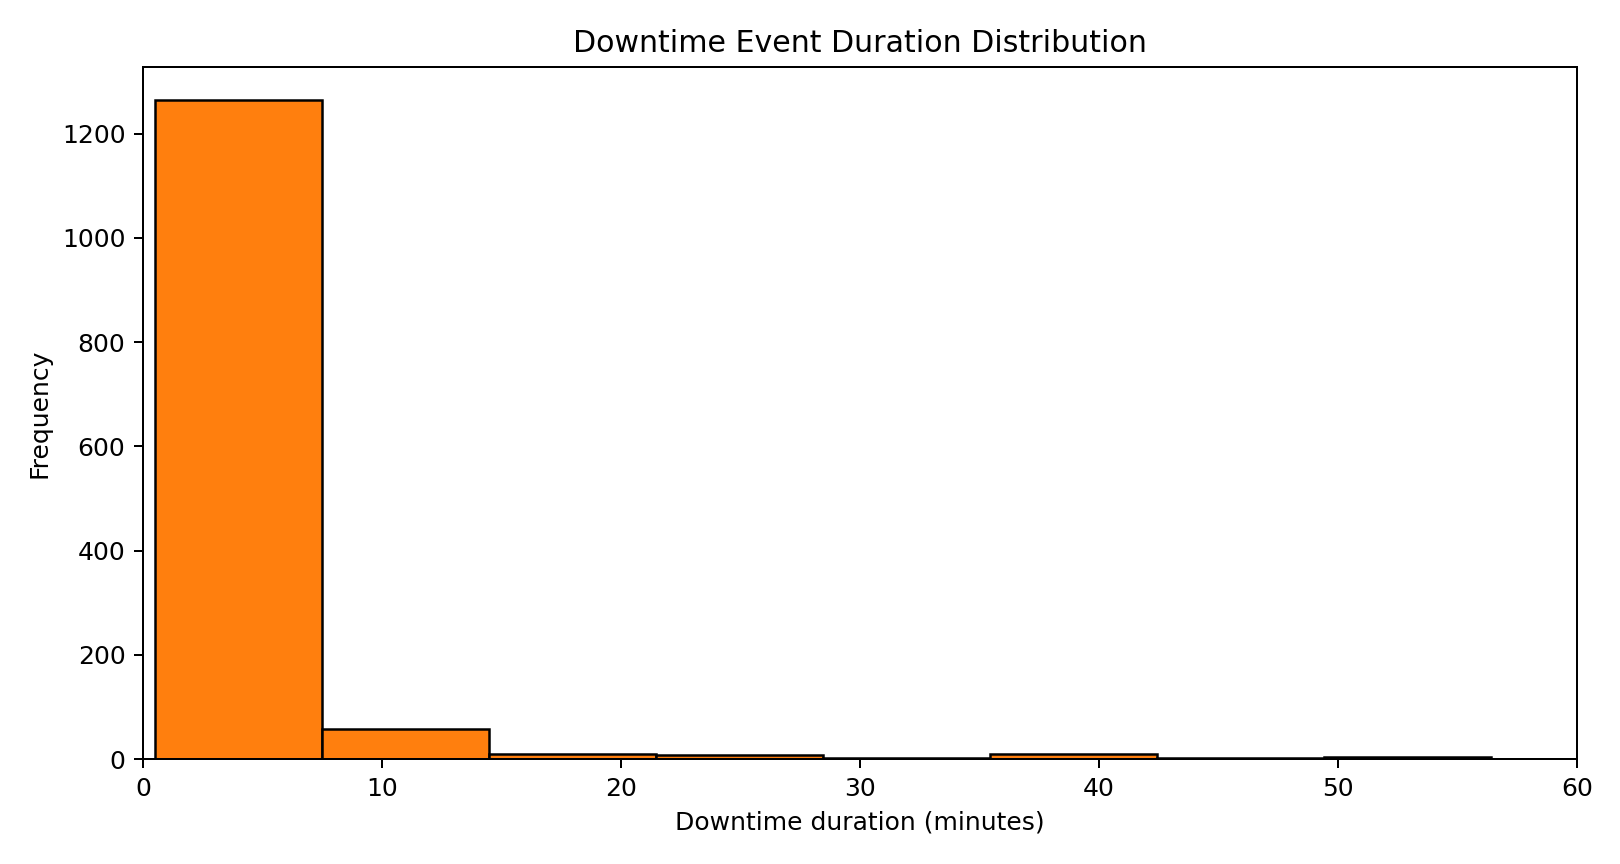
\includegraphics[width=\columnwidth]{outputs/downtime_distribution.png}
\caption{Distribution of downtime-event duration, truncated at 60 minutes for readability.}
\label{fig:dtdist}
\end{figure}

\begin{table}[!t]
\caption{Downtime Category Structure}
\label{tab:downtimecat}
\centering
\begin{tabular}{lrr}
\toprule
Category & Event Count & Share of Downtime Minutes \\
\midrule
Micro ($\leq$ 2 min) & 851 & 13.59\% \\
Minor (2--10 min) & 443 & 20.15\% \\
Major ($>$ 10 min) & 94 & 66.26\% \\
\bottomrule
\end{tabular}
\end{table}

\begin{figure}[!t]
\centering
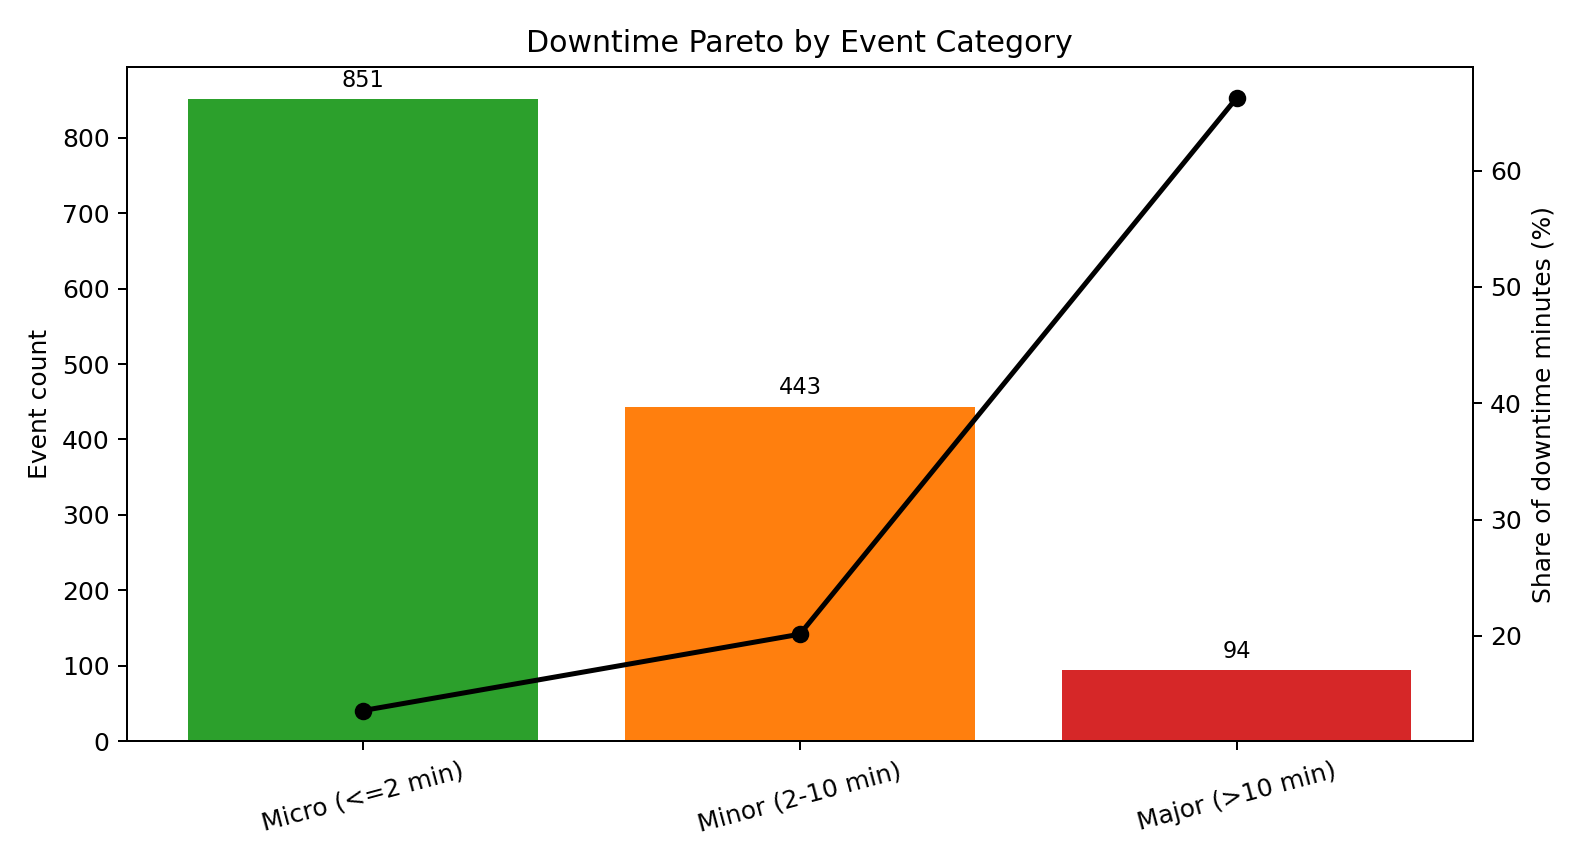
\includegraphics[width=\columnwidth]{outputs/downtime_category_pareto.png}
\caption{Downtime Pareto by event category. Major stoppages are rare but dominant in lost time.}
\label{fig:pareto}
\end{figure}

The data show that micro-stoppages account for 61.31\% of all events but only 13.59\% of lost time, whereas major stoppages account for just 6.77\% of events but consume 66.26\% of lost time. This is one of the central findings of the study because it explains why some lean strategies produce much larger gains than others.

\subsection{Relationship Between Pause Time and Efficiency}
Figure~\ref{fig:pauseeff} shows that higher pause time is associated with lower daily efficiency. The negative slope of the trend line confirms that the loss of productive operating time is a direct driver of productivity deterioration.

\begin{figure}[!t]
\centering
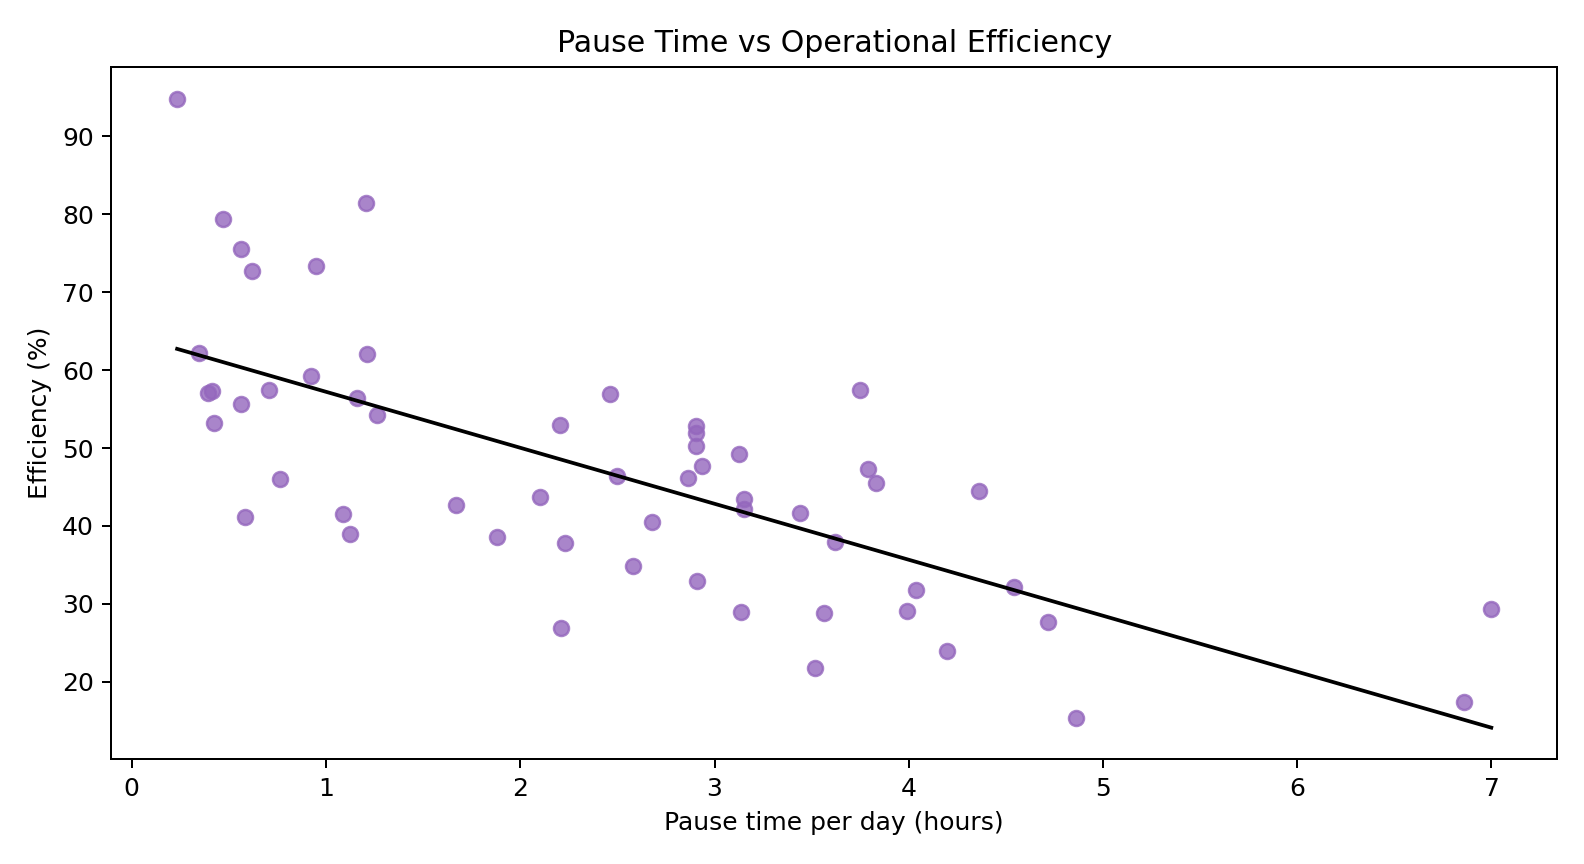
\includegraphics[width=\columnwidth]{outputs/pause_vs_efficiency.png}
\caption{Daily pause time versus operational efficiency.}
\label{fig:pauseeff}
\end{figure}

\subsection{Product-Level Production Rate Comparison}
Figure~\ref{fig:prodrate} compares the mean and median production rates for the two product sizes. The 5 L product shows a higher effective rate, indicating that product mix should be considered when future line-balancing or scheduling studies are carried out.

\begin{figure}[!t]
\centering
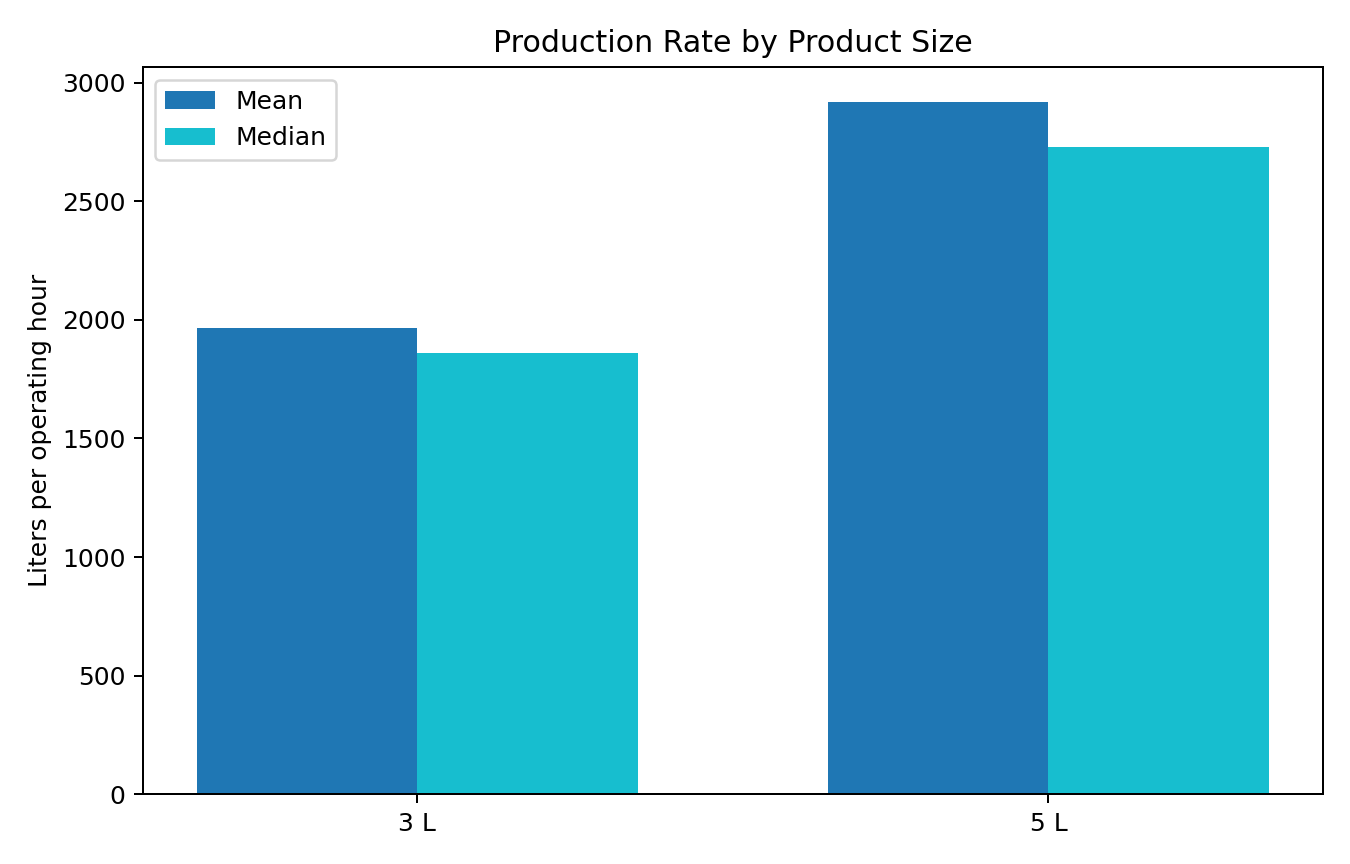
\includegraphics[width=\columnwidth]{outputs/product_rate_comparison.png}
\caption{Mean and median production rate by product size.}
\label{fig:prodrate}
\end{figure}

\subsection{Simulation Results}
The baseline simulation produced 211,924.69 liters on average over the resampled production horizon, which closely matches the observed output of the real system. This indicates that the model is a reasonable representation of the operating pattern captured in the dataset.

\begin{table}[!t]
\caption{Simulation Results for Lean Scenarios}
\label{tab:sim}
\centering
\begin{tabular}{lrrrr}
\toprule
Scenario & Mean Output (L) & Gain (\%) & Eff. (\%) & Eff. Gain (pp) \\
\midrule
Baseline & 211,924.69 & 0.00 & 42.37 & 0.00 \\
5S + Visual Management & 216,866.69 & 2.33 & 43.25 & 0.88 \\
TPM & 255,604.10 & 20.61 & 50.81 & 8.44 \\
Integrated Lean Bundle & 280,142.22 & 32.19 & 55.33 & 12.96 \\
\bottomrule
\end{tabular}
\end{table}

\begin{table}[!t]
\caption{Simulation Uncertainty Range}
\label{tab:uncertainty}
\centering
\begin{tabular}{lrr}
\toprule
Scenario & P05 Output (L) & P95 Output (L) \\
\midrule
Baseline & 188,572.81 & 236,799.79 \\
5S + Visual Management & 192,906.87 & 242,100.46 \\
TPM & 226,295.58 & 287,389.24 \\
Integrated Lean Bundle & 247,828.10 & 314,804.33 \\
\bottomrule
\end{tabular}
\end{table}

\begin{figure}[!t]
\centering
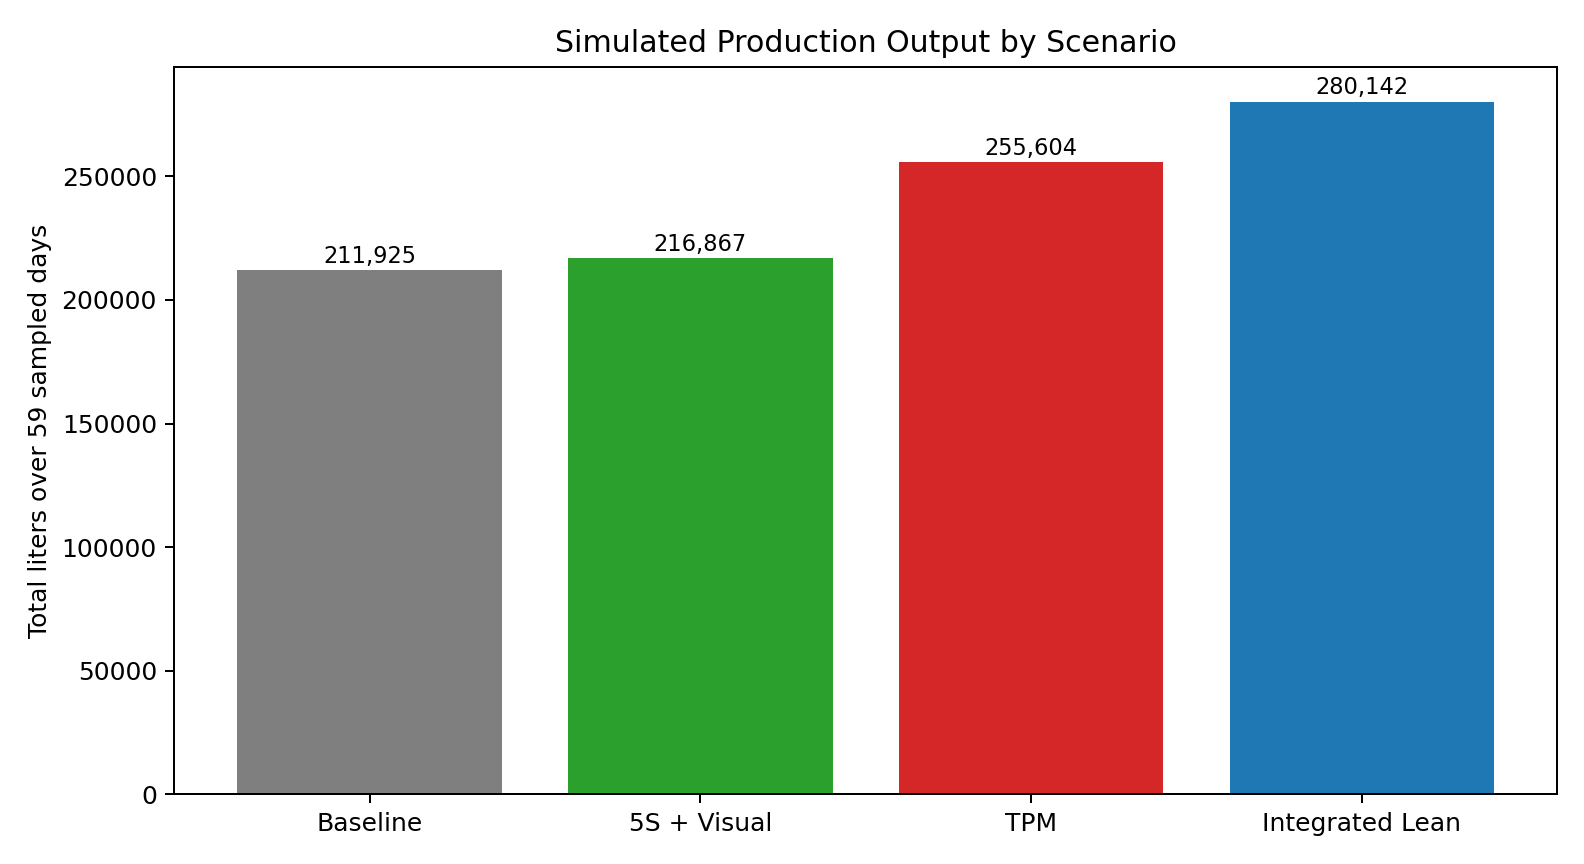
\includegraphics[width=\columnwidth]{outputs/scenario_output.png}
\caption{Mean simulated production output across the baseline and lean scenarios.}
\label{fig:scenariooutput}
\end{figure}

The 5S scenario produces a modest improvement because it targets frequent but low-duration stoppages. TPM produces a much stronger gain because it attacks the dominant lost-time source. The integrated lean bundle performs best because it reduces waste across all three downtime classes, especially the severe breakdown category.

\section{Discussion}
The results suggest that lean selection should be based on the structure of loss rather than on the visibility of problems. In many factories, micro-stoppages are more visible to supervisors because they happen frequently, but they may not be the main source of lost production. In the present case, TPM provides far more leverage than 5S because the underlying downtime distribution is highly concentrated in major stoppages.

This finding is aligned with the broader literature showing that lean tools are not equally powerful in every setting [1], [4], [5]. It also supports the argument that simulation is particularly valuable for SMEs, where incorrect prioritization is costly [3]. Instead of launching multiple improvement programs at once, the firm can use data to sequence actions more rationally.

The results also strengthen the connection between lean and digital manufacturing. Rather than using static value stream mapping alone, the study uses actual event-level operational data. This is consistent with the direction suggested by smart-manufacturing and digital-twin literature [6], [10]. For student projects, this is also important academically because it moves the work beyond a descriptive lean case study into quantitative industrial engineering research.

\section{Conclusion}
This paper developed an expanded simulation-based framework for evaluating lean manufacturing strategies using a real industrial bottling-line dataset. The analysis showed that the line suffers from low availability and a highly skewed downtime structure. Although micro-stoppages are the most frequent events, major stoppages dominate total lost time.

The simulation demonstrated that 5S and visual management improve output by 2.33\%, TPM improves output by 20.61\%, and an integrated lean bundle improves output by 32.19\% while raising simulated mean availability from 42.37\% to 55.33\%.

The managerial implication is straightforward: for this line, maintenance-led downtime reduction should be prioritized first, followed by broader workplace-stabilization measures such as 5S, standard work, and visual management. The academic implication is that open industrial data can be used to build reproducible lean-simulation studies suitable for SME-oriented manufacturing research.

\section*{Limitations and Future Scope}
The scenario reductions used in the simulation are literature-informed assumptions rather than observed post-implementation values. The dataset also does not provide root-cause-coded downtime labels, which limits the precision with which each downtime class can be mapped to a specific lean tool. Future work may extend the study by collecting cause-coded downtime data, quality-loss records, labor observations, and actual post-implementation shop-floor results.

\section*{Why the Earlier Draft Showed [?]}
The earlier file used LaTeX citation commands tied to an external bibliography database. When such a file is opened without running the full LaTeX bibliography workflow, unresolved references appear as ``[?]''. This expanded file avoids that problem by using fixed in-text reference numbers and a self-contained reference list.

\begin{thebibliography}{11}

\bibitem{r1}
I. Belekoukias, J. A. Garza-Reyes, and V. Kumar, ``The impact of lean methods and tools on the operational performance of manufacturing organisations,'' \emph{International Journal of Production Research}, vol. 52, no. 18, pp. 5346--5366, 2014, doi: 10.1080/00207543.2014.903348.

\bibitem{r2}
O. Oleghe and K. Salonitis, ``Hybrid simulation modelling of the human-production process interface in lean manufacturing systems,'' \emph{International Journal of Lean Six Sigma}, vol. 10, no. 2, pp. 665--690, 2019, doi: 10.1108/IJLSS-01-2018-0004.

\bibitem{r3}
F. Yu and Z. Chen, ``Tools, application areas and challenges of factory simulation in Small and Medium-Sized Enterprises -- A Review,'' \emph{Procedia CIRP}, vol. 104, pp. 399--404, 2021, doi: 10.1016/j.procir.2021.11.067.

\bibitem{r4}
J. Possik, A. Zouggar-Amrani, B. Vallespir, and G. Zacharewicz, ``Lean techniques impact evaluation methodology based on a co-simulation framework for manufacturing systems,'' \emph{International Journal of Computer Integrated Manufacturing}, vol. 35, no. 1, pp. 91--111, 2022, doi: 10.1080/0951192X.2021.1972468.

\bibitem{r5}
S. Frecassetti, B. Kassem, K. Kundu, M. Ferrazzi, and A. Portioli-Staudacher, ``Introducing Lean practices through simulation: A case study in an Italian SME,'' \emph{Quality Management Journal}, vol. 30, no. 2, pp. 90--104, 2023, doi: 10.1080/10686967.2023.2171326.

\bibitem{r6}
J. A. C. Bokhorst, W. Knol, J. Slomp, and T. Bortolotti, ``Assessing to what extent smart manufacturing builds on lean principles,'' \emph{International Journal of Production Economics}, vol. 253, art. no. 108599, 2022, doi: 10.1016/j.ijpe.2022.108599.

\bibitem{r7}
G. A. David, P. M. C. Monson, C. Soares Junior, P. O. Concei\c{c}\~ao Junior, P. R. Aguiar, and A. Simeone, ``IoT-Driven Deep Learning for Enhanced Industrial Production Forecasting,'' \emph{IEEE Internet of Things Journal}, vol. 11, no. 23, pp. 38486--38495, 2024, doi: 10.1109/JIOT.2024.3447579.

\bibitem{r8}
G. A. David, P. M. C. Monson, and C. Soares Junior, \emph{Industrial Production Time-Series Dataset from a Beverage Bottling Line}. Zenodo, Jan. 4, 2026. doi: 10.5281/zenodo.18146866.

\bibitem{r9}
J. M. Matindana and M. J. Shoshiwa, ``Lean manufacturing implementation in food and beverage SMEs in Tanzania: using structural equation modelling (SEM),'' \emph{Management System Engineering}, vol. 4, no. 1, pp. 1--14, 2025, doi: 10.1007/s44176-025-00036-3.

\bibitem{r10}
M. Reslan, M. J. Triebe, R. Venketesh, and A. J. Hartwell, ``Automation of Value Stream Mapping: A Case Study on Enhancing Lean Manufacturing Tools Through Digital Twins,'' \emph{Procedia CIRP}, vol. 134, pp. 455--460, 2025, doi: 10.1016/j.procir.2025.02.159.

\bibitem{r11}
C. Unal and S. Bilget, ``Examination of lean manufacturing systems by simulation technique in apparel industry,'' \emph{The Journal of The Textile Institute}, vol. 112, no. 3, pp. 377--387, 2021, doi: 10.1080/00405000.2020.1756104.

\end{thebibliography}

\end{document}
